\documentclass[letterpaper]{article}
\ifdefined\ANONBUILD
\usepackage[submission]{aaai2026}
\else
\usepackage{aaai2026}
\nocopyright
\fi
\usepackage{times}
\usepackage{helvet}
\usepackage{courier}
\usepackage[hyphens]{url}
\usepackage{graphicx}
\usepackage{placeins}
\urlstyle{rm}
\def\UrlFont{\rm}
\usepackage{natbib}
\usepackage{caption}
\frenchspacing
\setlength{\pdfpagewidth}{8.5in}
\setlength{\pdfpageheight}{11in}

\usepackage{amsmath,amssymb}
\usepackage{booktabs}
\usepackage{tabularx}
\newif\ifanonymoussubmission
\ifdefined\ANONBUILD
  \anonymoussubmissiontrue
\else
  \anonymoussubmissionfalse
\fi

\newcommand{\system}{TRACE-RPG}
\newcommand{\Valid}{\mathrm{valid}}
\newcommand{\AcceptSet}{\mathcal{A}}
\newcommand{\GoalSet}{\mathcal{G}}
\newcommand{\HitSet}{\mathcal{H}}
\newcommand{\SchemaSet}{\mathcal{S}}
\newcommand{\RepoURL}{\ifanonymoussubmission [Anonymous Repository URL withheld for double-anonymous review]\else \url{https://github.com/akillness/neural_symbolic_in_game}\fi}
\AtBeginDocument{\emergencystretch=2.5em}
\providecommand{\Description}[2][]{}


\setcounter{secnumdepth}{1}

\title{TRACE-RPG: Auditable Proposal-to-Commit Boundaries for Narrative Mediation and Game State Authorization}
\author{
  Jangyoung Jeong\textsuperscript{\rm 1},
  Shinjin Kang\textsuperscript{\rm 2}\thanks{Corresponding author.}
}
\affiliations{
  \textsuperscript{\rm 1}Department of Game Design, Hongik University\\
  \textsuperscript{\rm 2}Hongik University
}

\begin{document}
\maketitle

\begin{abstract}
Generated game events can satisfy a syntactic schema and cite known facts while requesting inaccessible objects, unauthorized state transitions, or premature secret disclosure. \system{} separates proposal authority from commit authority at a deterministic seven-predicate gate backed by Theorems~1--4 for invariants \textbf{I1--I4}. Across 1,664 finite-graph cases, semantic gating eliminated 260/416 schema-only unsafe commits (0/156 false rejections; 128/260 guided repairs), and a 48-case multi-hop closure suite breaks 60/60 single-hop parity (\texttt{ontology\_}\allowbreak\texttt{multihop\_}\allowbreak\texttt{gate} 48/48 vs.\ flat 20/48). Across 24 live Antigravity CLI Gemini episodes over three quests, zero unsafe commits occurred (70 schema-unsafe turns blocked, 24/24 strict replay, CLI revisions unattested), while Stage-2 EN/KO escape verification reaches 97.2\% paraphrase recall at 0.0\% benign false rejection alongside extended zero-LLM audits and a blinded \texttt{TR01--TR06} human-eval packet (\texttt{AWAITING\_}\allowbreak\texttt{HUMAN\_}\allowbreak\texttt{RATERS}).
\end{abstract}

\section{Introduction}
Generated game events can satisfy a syntactic schema and cite known facts while requesting inaccessible objects, unauthorized state changes, or premature secret disclosure. Grounding and plausible dialogue \cite{S03_weir2024ontologically,S20_ashby2023personalized} supply candidate content, yet the game engine must still decide which state transitions to authorize.

\system{} enforces this decision at an external proposal-to-commit boundary (Fig.~\ref{fig:architecture}). Models and adapters submit typed candidates to a deterministic gate that checks action policies, preconditions, object reachability, NPC knowledge, disclosure permissions, effects, and quest-stage monotonicity. When a check fails, the gate returns structured errors for bounded repair; repair modifies only the candidate rather than canonical state, and mutation occurs only after same-state revalidation. A read-only eight-role ontology view links source declarations to these checks and public decisions without write authority, while hash-linked transition records support semantic replay and assignment-complete accounting.

Conceptually, this contract goes beyond factual grounding by separating an NPC's \emph{epistemic knowledge boundary} (facts an actor knows) from its \emph{disclosure authorization policy} (facts an actor may reveal at the current quest stage). Methodologically, our evaluation separates a zero-LLM-call deterministic verification layer (gate checks, guided repair, and engine replay) from a bounded stochastic proposer layer with explicit failure retention.

Across our deterministic audits, a schema-only baseline committed 260/416 reference-invalid proposals across 32 finite-graph configurations, whereas all semantic-gate arms recorded 0/416 unsafe commits while preserving 156/156 valid proposals ($0/156$ false rejections) and 11/11 structural signatures; guided repair recovered 128/260 invalid proposals. In single-hop disclosure checks, general-rule and ontology-gate implementations agreed on 60/60 cases while eliminating 51 unique unsafe disclosures from an unchecked baseline; a subsequent 48-case multi-hop closure benchmark separates them cleanly (\texttt{ontology\_}\allowbreak\texttt{multihop\_}\allowbreak\texttt{gate} 48/48 vs.\ \texttt{flat\_}\allowbreak\texttt{1hop\_}\allowbreak\texttt{rule} 20/48, preventing 28 leaks). Extended zero-LLM audits, Theorems~1--4 for invariants \textbf{I1--I4}, a 24-episode live multi-quest Gemini evaluation (2/2 models, 3 worlds, 0 unsafe commits, 24/24 strict replay), Stage-2 EN/KO escape verifiers (97.2\% paraphrase recall at 0.0\% benign false rejection), and a trace-bound 36-item human-evaluation packet (\texttt{AWAITING\_}\allowbreak\texttt{HUMAN\_}\allowbreak\texttt{RATERS}) with Croissant~1.0 metadata complete our reproducible release boundary.

\section{Related Work and Research Gap}
Grounding, memory, planning, and role-based agents \cite{S03_weir2024ontologically,S20_ashby2023personalized,S07_park2023generative,S08_shao2023character}, together with player and dialogue systems \cite{S21_akoury2023player,S22_hochreiter2026beyond,S23_yin2026contextualized,S02_figueiredo2025scaffolded}, support contextual interaction, whereas we examine whether the current encoded state and disclosure policy permit a proposed transition. Modeling affect and engagement \cite{S24_yannakakis2011experiencedriven,S25_melhart2020engagement,S26_wang2026engagement} targets different outcomes: style preferences, affect estimates, and personality labels may guide generation but do not authorize state mutations.

Existing benchmarks and automated play-testing cover state, embodiment, content, process, social interaction, and long-horizon play \cite{S11_cote2019textworld,S12_wang2022scienceworld,S13_fan2022minedojo,S14_perezliebana2019gvgai,S15_liu2024agentbench,S16_ma2024agentboard,S17_zhou2024sotopia,S18_paglieri2025balrog,S19_lepelletier2022playtesting}, while NCP-Bench evaluates narrative commitment and fact consistency \cite{S58_ma2026ncpbench}. Structural, schema, affordance, and neuro-symbolic rule methods motivate our constraint design \cite{S09_geng2023grammar,S10_beurerkellner2023prompting,S36_scholak2021picard,S50_kambhampati2024llmmodulo,S51_ichter2023saycan,S52_wang2025agentspec,S53_li2025settingdc,S54_zhou2025story2game,S42_buongiorno2024pangea}, alongside counterexample-guided repair \cite{S45_madaan2023selfrefine,S48_shinn2023reflexion,S46_chen2023selfdebug,S47_solarlezama2006sketching} and reproducibility/accounting standards \cite{S31_agarwal2021precipice,S33_pineau2021reproducibility,S56_feng2025agentrr,S59_sun2025bdc}. Unlike prior systems that conflate schema validity with action legality or treat factual grounding as sufficient for dialogue safety, \system{} isolates schema parsing, epistemic knowledge, disclosure permission, and canonical state commit into separately auditable gates.


\begin{figure*}[!t]
  \centering
  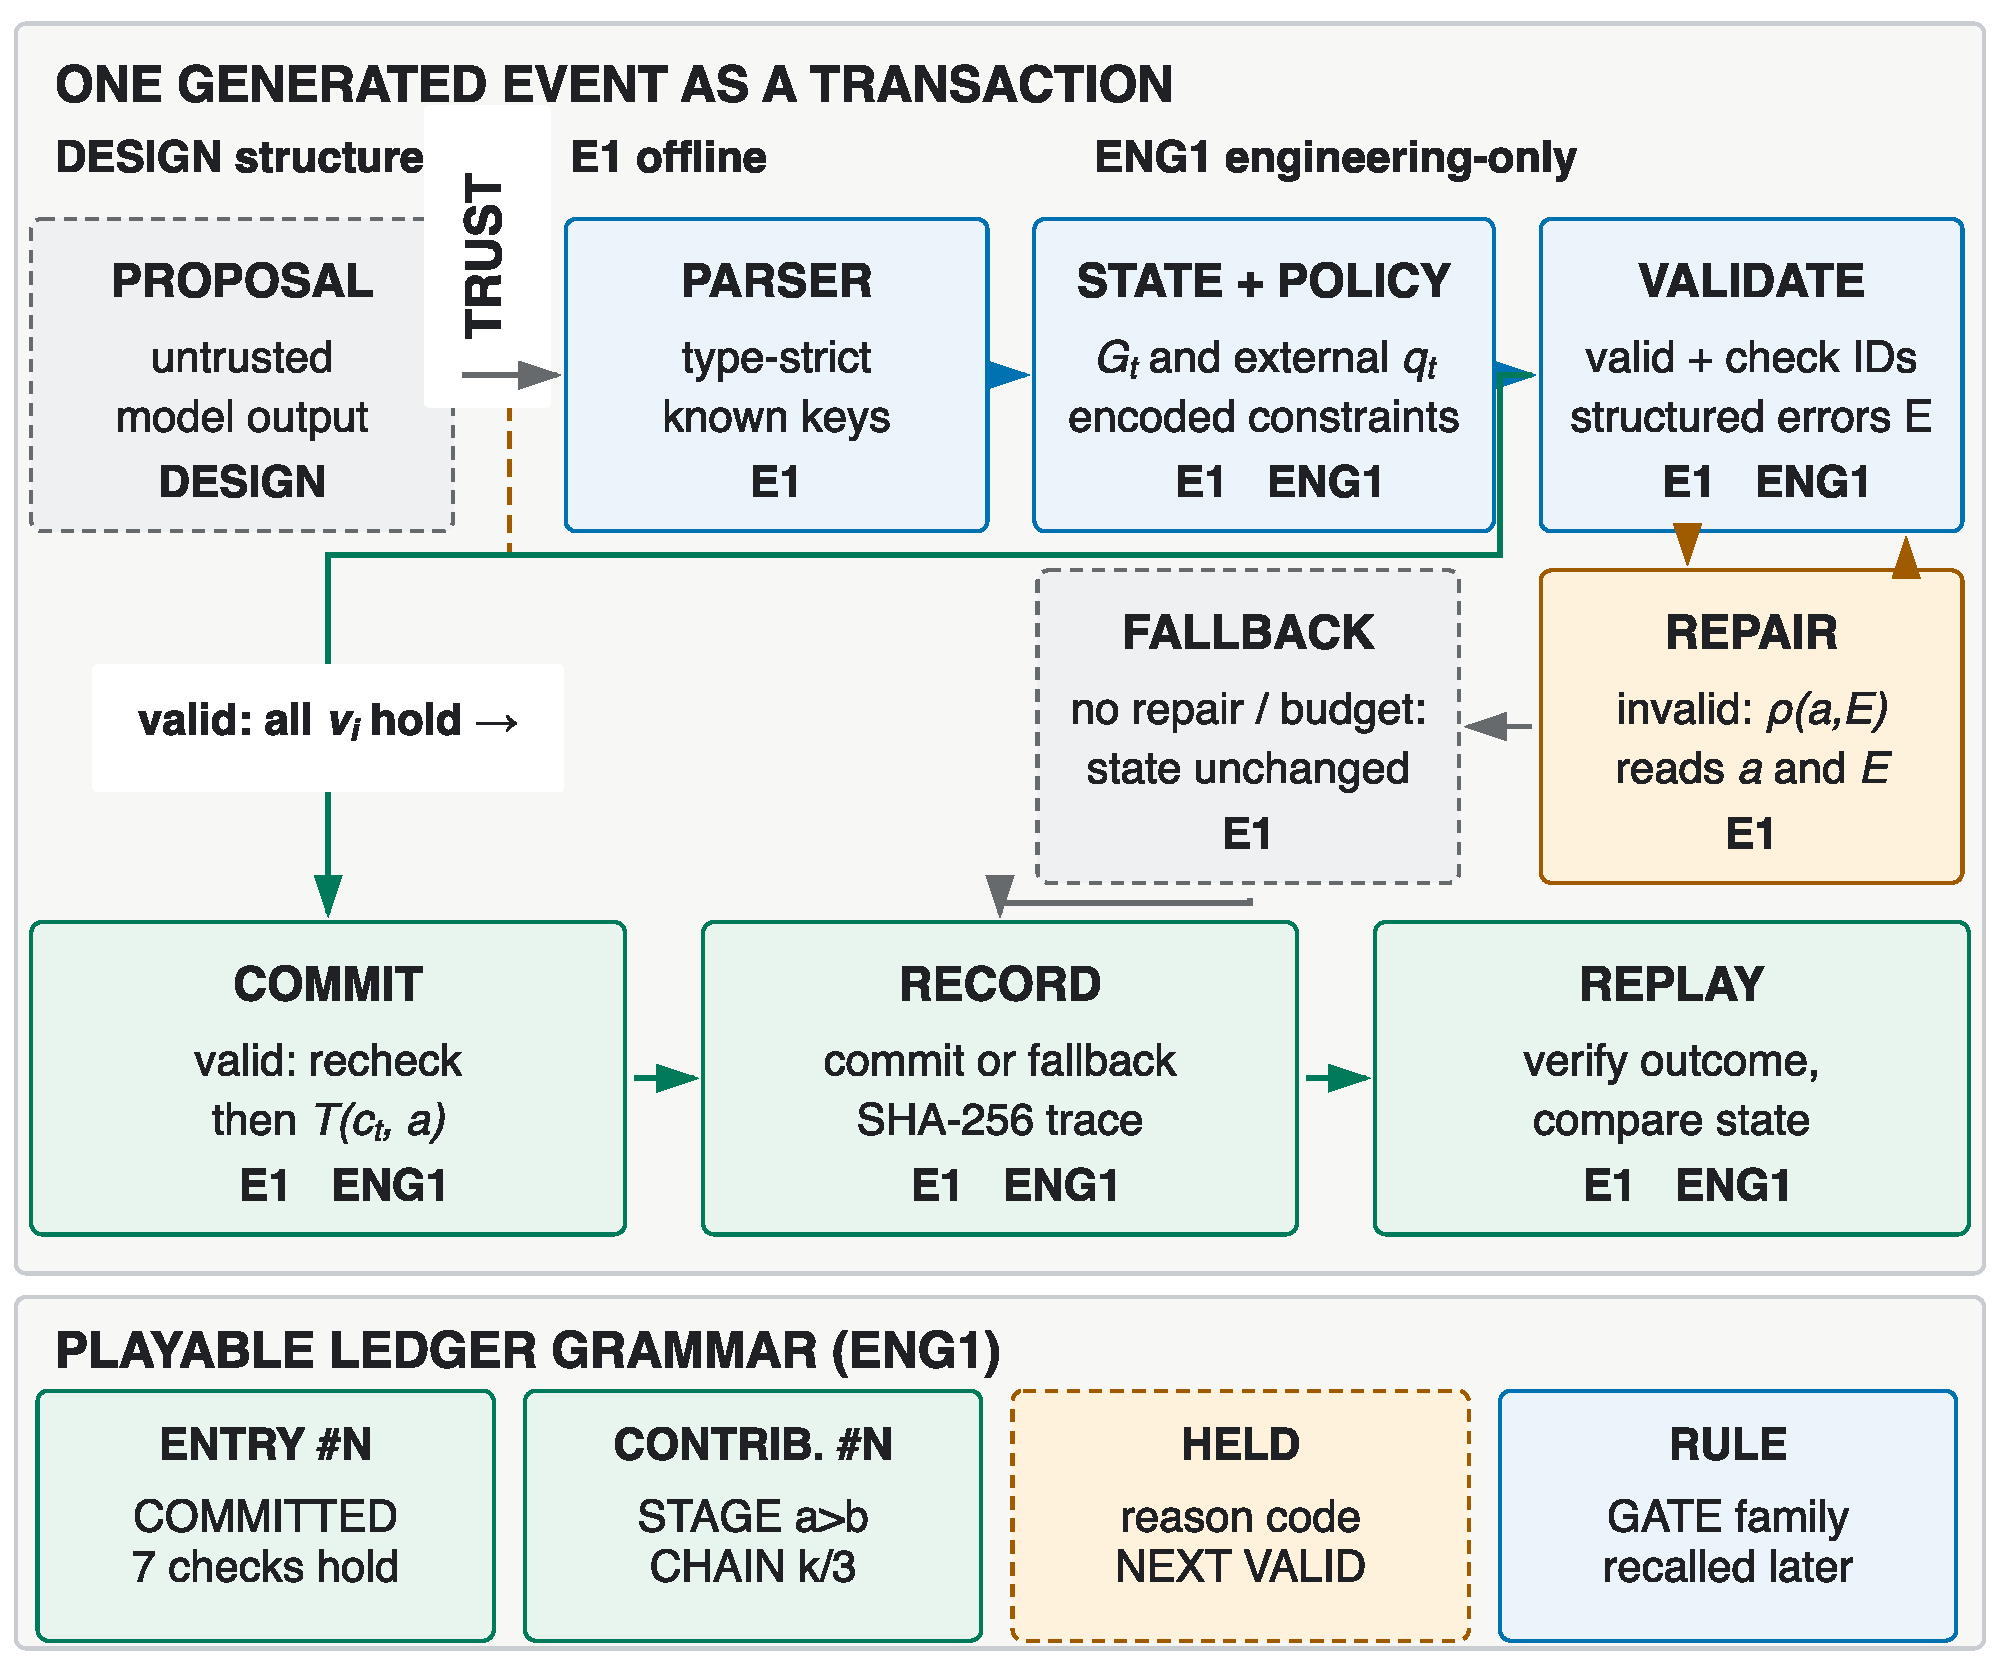
\includegraphics[width=0.72\textwidth]{../../figures/fig_architecture.pdf}
  \caption{Policy and state $c_t$ gate proposals; errors feed bounded $\rho$ or unchanged fallback before revalidated commit and replay.}
  \label{fig:architecture}
\end{figure*}

\section{Problem Definition and Guarantee Boundary}\label{sec:problem}
In $c_t=(G_t,q_t)$, $G_t$ denotes the typed game snapshot (locations, reachable locations, object placements, inventory, facts, NPC knowledge, and quest stage) and $q_t$ contains externally authored action-policy, disclosure, and quest-stage constraints. Predicates neither reconstruct history $h_{<t}$ nor mutate $q_t$, and retrieval outputs or affect scores carry zero write authority.

After strict schema parsing of an untrusted proposal $a_t$, the validator runs seven deterministic predicates and returns \texttt{Validation}\allowbreak\texttt{Result}(\allowbreak$\mathrm{valid},E_t,C_{\mathrm{run}}$):
\begin{equation}
\begin{aligned}
V(c_t,a_t)&=(\mathrm{valid},E_t,C_{\mathrm{run}}),\\
\boldsymbol{v}&=(v_{\mathrm{policy}},v_{\mathrm{pre}},v_{\mathrm{reach}},\\
&\qquad v_{\mathrm{know}},v_{\mathrm{disc}},v_{\mathrm{elig}},v_{\mathrm{stage}})\in\{0,1\}^{7},
\end{aligned}
\end{equation}
where $\mathrm{valid}\equiv\bigwedge_{i=1}^{7}(v_i=1)$ and $E_t$ records typed error codes, entities, reasons, and repair hints. Canonical state updates only when all seven predicates pass:
\begin{equation}
c_{t+1}=\begin{cases}
T(c_t,a_t), & \bigwedge_{i=1}^{7}(v_i=1),\\
c_t, & \text{otherwise.}
\end{cases}
\label{eq:transition}
\end{equation}

\subsection{Schema Validity, Authorization, and Goal Success}\label{sec:authorization-sets}
Fix the pre-action state $c_t$, authored policy, and strict schema. Let $\SchemaSet$ be the set of schema-valid candidates; we separate authorization from goal attainment:
\begin{equation}
\begin{aligned}
\AcceptSet(c_t)&=\{a\in\SchemaSet:V(c_t,a).\mathrm{valid}\},\\
\GoalSet(c_t)&=\{a\in\SchemaSet:\operatorname{Goal}(T(c_t,a))\},\\
\HitSet(c_t)&=\AcceptSet(c_t)\cap\GoalSet(c_t)\subseteq\AcceptSet(c_t)\subseteq\SchemaSet.
\end{aligned}
\end{equation}
A schema-valid candidate that declares a forbidden fact falls outside $\AcceptSet$, whereas a permitted observation action can lie inside $\AcceptSet$ yet outside $\GoalSet$. Knowledge and disclosure permission are independent inputs: an NPC can know \texttt{keeper\_\allowbreak secret} at both stage $0$ and stage $1$ while disclosure is forbidden at stage $0$ and permitted at stage $1$.

\subsection{Formal Security Theorems for Invariants I1--I4}\label{sec:formal-proofs}
Under Eq.~\eqref{eq:transition} and strict parser \texttt{parse\_}\allowbreak\texttt{candidate\_}\allowbreak\texttt{mapping}, invariants \textbf{I1--I4} hold as conditional structural theorems over any finite encoded state $c_t=(G_t,q_t)$, repair budget $K\in\mathbb{Z}_{\geq 0}$, and returning callbacks:

\noindent\textbf{Theorem 1 (I1: State-Preservation Safety).} \emph{If the initial candidate fails strict parsing or all $K{+}1$ candidates yield $V(c_t,a^{(j)}).\mathrm{valid}=\mathrm{false}$, then $c_{t+1}=c_t$ and committed effects are empty.}
\par\noindent\textit{Proof.} \texttt{parse\_}\allowbreak\texttt{candidate\_}\allowbreak\texttt{mapping} rejects malformed proposals prior to commit; in Fig.~\ref{alg:commit}, $\operatorname{Commit}$ is reachable only on $\mathrm{ok}=\mathrm{true}$, while $j=K$ invokes $\operatorname{Fallback}(c_t)$ returning $c_t$ untouched by Eq.~\eqref{eq:transition}. \hfill$\square$

\noindent\textbf{Theorem 2 (I2: Bounded Termination and State-Blind Anti-Laundering Repair).} \emph{For any finite $K{\geq}0$ and returning callbacks, the loop executes at most $K{+}1$ validator calls, revalidates $V(c_t,a^{(j)})$ immediately prior to mutation, and never alters \texttt{WorldState}-dependent authorization classes under $\rho$.}
\par\noindent\textit{Proof.} Loop counter $j$ starts at $0$, checks $j=K$ before incrementing, and halts on $\mathrm{ok}=\mathrm{true}$ or $j=K$, bounding $V$ calls by $K{+}1$. By Table~\ref{tab:rho-rules}, $\rho(a,E)$ inspects only $(a,E)$ without reading \texttt{WorldState} and maps \texttt{UNKNOWN\_}\allowbreak\texttt{ACTION\_}\allowbreak\texttt{TYPE}, \texttt{UNREACHABLE\_}\allowbreak\texttt{REQUIRED\_}\allowbreak\texttt{OBJECT}, \texttt{NPC\_}\allowbreak\texttt{KNOWLEDGE\_}\allowbreak\texttt{VIOLATION}, \texttt{NPC\_}\allowbreak\texttt{DIS\-CLOSURE\_}\allowbreak\texttt{KNOW\-LEDGE\_}\allowbreak\texttt{VIO\-LATION}, \texttt{FORBIDDEN\_}\allowbreak\texttt{DISCLOSURE}, \texttt{QUEST\_}\allowbreak\texttt{STAGE\_}\allowbreak\texttt{VIOLATION}, and \texttt{QUEST\_}\allowbreak\texttt{STAGE\_}\allowbreak\texttt{REGRESSION} to identity while dropping same-field conflicts. \hfill$\square$

\noindent\textbf{Theorem 3 (I3: Policy-Bounded Mutation).} \emph{Every committed state transition satisfies all seven predicates $v_1\dots v_7$ and applies only effects permitted by \texttt{ActionPolicy.}\allowbreak\texttt{allowed\_}\allowbreak\texttt{effects}.}
\par\noindent\textit{Proof.} Strict parsing freezes the 12 \texttt{CANDIDATE\_}\allowbreak\texttt{FIELDS}; $v_{\mathrm{policy}}{=}1$ verifies effect membership in \texttt{allowed\_}\allowbreak\texttt{effects} and $T$ writes no undeclared keys. \hfill$\square$

\noindent\textbf{Theorem 4 (I4: Deterministic Semantic Replay).} \emph{Given ordered hash-chained transition records with \texttt{allow\_}\allowbreak\texttt{defaults=false} parsing and frozen $(V,T)$, replaying proposals from $c_0$ uniquely reconstructs $c_T$ and detects any single-step tampering via SHA-256 chain mismatch.}
\par\noindent\textit{Proof.} Both $V$ and $T$ are pure deterministic functions of $(c_t,a_t)$, and each record hashes $(\mathrm{hash}(c_t),\allowbreak a_t,\allowbreak V(c_t,a_t),\allowbreak\mathrm{hash}(c_{t+1}))$; inductive agreement from $c_0$ yields $\mathrm{hash}(c'_T)=\mathrm{hash}(c_T)$. \hfill$\square$

\section{TRACE-RPG Architecture and Algorithms}\label{sec:arch}
Models and adapters propose candidate actions, the strict parser rejects unknown keys and ambiguous types, and a versioned bridge carries observations, proposals, validations, rejections, fallbacks, and commits (Fig.~\ref{fig:architecture}, Table~\ref{tab:validators}). An eight-role read-only ontology view (\texttt{World}, \texttt{Actor}, \texttt{Knowledge}, \texttt{Fact}, \texttt{Policy}, \texttt{Quest}, \texttt{Action}, \texttt{Trace}) maps source declarations to executed checks and replay receipts without granting mutation authority.

\begin{table}[!tbp]
\caption{Encoded Seven-Predicate Validator Boundary}
\label{tab:validators}
\centering
\footnotesize
\begin{tabularx}{\columnwidth}{@{}>{\raggedright\arraybackslash}p{0.26\columnwidth}>{\raggedright\arraybackslash}X>{\raggedright\arraybackslash}p{0.18\columnwidth}@{}}
\toprule
\textbf{Predicate} & \textbf{Rejects} & \textbf{On failure} \\
\midrule
Action policy & unknown action/type; omitted required preconditions/effects; disallowed effects & unchanged \\
Precondition & absent or false requirement & unchanged \\
Reachability & inaccessible target object & unchanged \\
NPC knowledge & used/disclosed fact absent from actor knowledge & unchanged \\
Disclosure & declared forbidden fact & unchanged \\
Quest stage & required stage above current stage & unchanged \\
Stage monotonicity & regressive quest-stage mutation & unchanged \\
\bottomrule
\end{tabularx}
\end{table}

\begin{figure}[!tbp]
\centering
\footnotesize
\begin{tabular}{@{}rl@{}}
1: & $a\leftarrow\operatorname{Propose}(c)$; $j\leftarrow0$ \\
2: & \textbf{repeat} \\
3: & \quad $(\mathrm{ok},E)\leftarrow V(c,a)$; $\operatorname{Record}(a,E)$ \\
4: & \quad \textbf{if} $\mathrm{ok}$ \textbf{then assert} $V(c,a).\mathrm{ok}$; \textbf{return} $\operatorname{Commit}(c,a)$ \\
5: & \quad \textbf{if} $j=K$ \textbf{then return} $\operatorname{Fallback}(c)$ \\
6: & \quad $a\leftarrow\operatorname{Repair}(c,a,E)$; $j\leftarrow j+1$ \\
7: & \textbf{until terminal}
\end{tabular}
\caption{Validate--Repair--Commit records at most $K+1$ candidate attempts and revalidates before mutation.}
\Description{Pseudocode of the Validate-Repair-Commit loop bounding validator calls to K+1 and revalidating prior to commit.}
\label{alg:commit}
\end{figure}

The guided repair operator $\rho(a,E)=a\oplus\bigcup_{e\in E}\delta(e)$ (Fig.~\ref{alg:commit}, Table~\ref{tab:rho-rules}) receives only candidate $a$ and structured errors $E$, never \texttt{WorldState}, preventing state laundering on reachability, knowledge, or disclosure violations. Transition records chain unkeyed SHA-256 hashes over prior state, candidate, validation outcome, and recomputed final state for deterministic semantic replay and assignment-complete denominator accounting.

\begin{table}[!tbp]
\caption{Per-Error-Class Edits of Guided Repair $\rho(a,E)$}
\label{tab:rho-rules}
\centering
\footnotesize
\begin{tabularx}{\columnwidth}{@{}>{\raggedright\arraybackslash}X>{\raggedright\arraybackslash}X@{}}
\toprule
\textbf{Validator error class} & \textbf{Edit $\delta(e)$ on candidate $a$} \\
\midrule
Policy precondition / effect omission & insert named predicate or effect \\
Policy effect violation & drop disallowed effect \\
Unsatisfied precondition & drop named predicate \\
Unauthorized stage mutation & clear \texttt{quest\_stage\_effect} \\
Unknown action; reachability, knowledge, disclosure, or stage classes & no-op (prevents state laundering) \\
\bottomrule
\end{tabularx}
\end{table}

\section{Evaluation}\label{sec:eval}
We organize evaluation into two non-pooled layers: (i) zero-LLM-call deterministic audits over finite graphs, disclosure matrices, link-prediction simulations, and Godot~4.7.1 engine execution, and (ii) bounded stochastic proposer pilots with strict assignment-complete denominators.

\subsection{Deterministic Authorization-Boundary Audit}
To test authorization beyond single-world unit fixtures, we cross two room counts (4, 8), two topologies (locked chain, unlocked bypass branch), four start/goal placements of two reusable keys, and two quest stages ($2{\times}2{\times}4{\times}2=32$ combinations) with 13 candidate variants each, yielding 416 assignments per arm (1,664 total) plus 48 separate surface-sentinel assignments (12/arm). An implementation-separated reference evaluates all initial and repaired candidates against the immutable pre-action state using standard-library BFS reachability.

\begin{table}[!tbp]
\caption{Deterministic Authorization-Boundary Audit (416 Cases/Arm + 48 Surface Sentinels; 0 LLM Calls)}
\label{tab:boundary-compact}
\centering
\footnotesize
\setlength{\tabcolsep}{3.5pt}
\begin{tabularx}{\columnwidth}{@{}>{\raggedright\arraybackslash}X*{4}{c}@{}}
\toprule
\textbf{Outcome (416/arm)} & \textbf{Schema} & \textbf{Sem.\ rej.} & \textbf{Retry} & \textbf{Guided $\rho$} \\
\midrule
Invalid initial proposals & 260 & 260 & 260 & 260 \\
Unsafe final commits & 260 & \textbf{0} & \textbf{0} & \textbf{0} \\
Repaired invalid $\rightarrow$ valid & 0 & 0 & 0 & \textbf{128} \\
Held (unchanged fallback) & 0 & 260 & 260 & 132 \\
Goal reached & 124 & 124 & 124 & \textbf{252} \\
Valid preserved (156 valid) & 156 & 156 & 156 & 156 \\
Signature retention (11 sigs) & 11/11 & 11/11 & 11/11 & 11/11 \\
\bottomrule
\end{tabularx}
\end{table}

Table~\ref{tab:boundary-compact} shows that \texttt{schema\_only} committed all 260/416 reference-invalid proposals, whereas every semantic-gate arm committed 0/416 invalid proposals with 0/156 false rejections and 32/32 closure--BFS agreement. Guided repair $\rho$ recovered 128/260 invalid proposals, nearly doubling goal attainment (252/416 vs.\ 124/416). On the 12/arm surface sentinels, all semantic gates blocked 6/6 explicit forbidden-fact declarations but admitted 6/6 undeclared paraphrases, quantifying the exact boundary of declared-field gating.

\subsection{Disclosure Parity and Ontology Link Simulation}
On 60 authored \texttt{reveal\_hint} cases (48 normal, 4 boundary, 8 malformed), an unchecked baseline produced 51 unique unsafe disclosures (60/60 allow), whereas \texttt{general\_rule} and \texttt{ontology\_gate} agreed on 60/60 outcomes (16 allow, 44 deny, 0 unsafe, 0 replay mismatches). This establishes zero-regression audit binding rather than ontology superiority over flat rules. Separately, in a closed-world KG link-proposal simulation (43 OKF nodes, 106 reference edges, 24 curated typed edges, 6 withheld-edge queries), typed-lexical retrieval (\texttt{S2}) achieved $P{=}R{=}1.000$, $\mathrm{MRR}{=}0.944$, and $\mathrm{Sem@3}{=}1.000$ versus degree baseline $P{=}R{=}0.000$ and $\mathrm{MRR}{=}0.282$.

\subsection{Extended Zero-LLM Engineering Audits (A1--A4, B)}
Table~\ref{tab:extended-compact} summarizes five independent-denominator audits covering multi-error convergence, scaling, traceability, Godot~4.7.1 soak stability, and secondary escape filtering.
\begin{table*}[!tbp]
\caption{Independent-Denominator Zero-LLM Engineering Audits (A1--A4, B)}
\label{tab:extended-compact}
\centering
\footnotesize
\begin{tabularx}{\textwidth}{@{}>{\raggedright\arraybackslash}p{0.20\textwidth}>{\raggedright\arraybackslash}p{0.21\textwidth}>{\raggedright\arraybackslash}X@{}}
\toprule
\textbf{Audit} & \textbf{Denominator / Scope} & \textbf{Verified Deterministic Results (0 LLM Calls)} \\
\midrule
\textbf{A1} Multi-Error Convergence & 352 cases/budget ($K{\in}\{0..3\}$, 1,408 runs) + 128 guards & Safe commits: $K{=}0$ 0/352, $K{\ge}1$ 124/352 (35.23\%, unsafe 0/1,408); \texttt{repairable\_multi} 96/96 at $K{=}1$; \texttt{mixed\_partial\_clear} 28/160 at $K{=}1$, 132/160 held; \texttt{conflict\_pair} 0/96 cross-attempt commits (96/96 period-2 oscillation at $K{=}3$) vs.\ 128/128 same-pass conflict-guard freeze. \\
\textbf{A2} Scaling Benchmark & $N{\in}[10,2000]$ facts ($\text{arity}{\le}100$ above 500), $R{\in}[4,256]$ rooms & At $N{=}2000$: validator p95 0.0042\,ms (valid) / 0.0751\,ms (multi-error); $\rho$ p95 0.0317--0.0389\,ms; $R{=}256$ closure/BFS p95 0.312--0.478\,ms; SHA-256 verify 7.01\,ms; JSONL replay ($N{=}100,L{=}100$) 881.0\,ms. \\
\textbf{A3} Traceability Faults & 4,656 seeded faults (+1,584 N/A), 3,744 invariance, \texttt{TR05} map & Seeded sensitivity 4,656/4,656 (100.00\%); invariance false alarms 0/3,744 (0.00\%); \texttt{TR05} forward 12/12, reverse 10/10 direct files; human Krippendorff $\alpha$ unmeasured (0 human raters). \\
\textbf{A4} Godot~4.7.1 Soak & 11 refusals + 1,600 ticks (200 episodes) & Refusal codes 9/9 (100\%) exercised; state isolation 11/11; trace consistency 1,600/1,600; \texttt{step\_commit} p95 0.708\,ms; static memory delta $-268$\,B; 0 leaks. \\
\textbf{B} Escape Filter (EN/KO) & 88 cases (44 EN, 44 KO; \texttt{keeper\_secret}) & Recall / benign FRR / warm p95: ID-only 0.0\% / 0.0\% / 0.032\,ms; Alias 61.1\% (22/36) / 11.1\% (4/36) / 0.041\,ms; LOO TF-IDF 97.2\% (35/36) / \textbf{58.3\% (21/36)} / 0.705\,ms. \\
\bottomrule
\end{tabularx}
\end{table*}

\subsection{Bounded Stochastic Proposer Pilots}
Across two small, non-confirmatory proposer collections, strict denominator accounting retains every parser and harness failure:
\begin{itemize}
\item \textbf{v5 Two-Stage Collection (20 assignments):} Crossing 5 synthetic fixtures $\times$ 2 selectors $\times$ Detailed/Generic feedback ($K{=}0$), 20/20 responses arrived, 10/20 passed strict parsing (Luna 9/10; Terra 1/10), 8/20 passed the semantic gate (all 2 rejected parsed outputs fell back safely with 0 mutations), and 7/20 reached \texttt{signal\_restored} (Fig.~\ref{fig:paired-feedback-flow}).
\item \textbf{Native Fixed-Quest Pilot (8 assignments):} On \texttt{sealed-\allowbreak lighthouse-\allowbreak v1} ($2\text{ selectors}\times 2\text{ representations}\times 2\text{ repeats}$), 5/8 reached the goal with 0/16 unsafe commits, 7/7 semantic replays valid, and 6/6 committed fresh Godot re-executions valid; 1 row failed pre-response serialization (controller-v3, fixed to v4 in rows 2--8) and 2 ontology rows timed out at 60\,s.
\end{itemize}

\begin{figure}[!tbp]
\centering
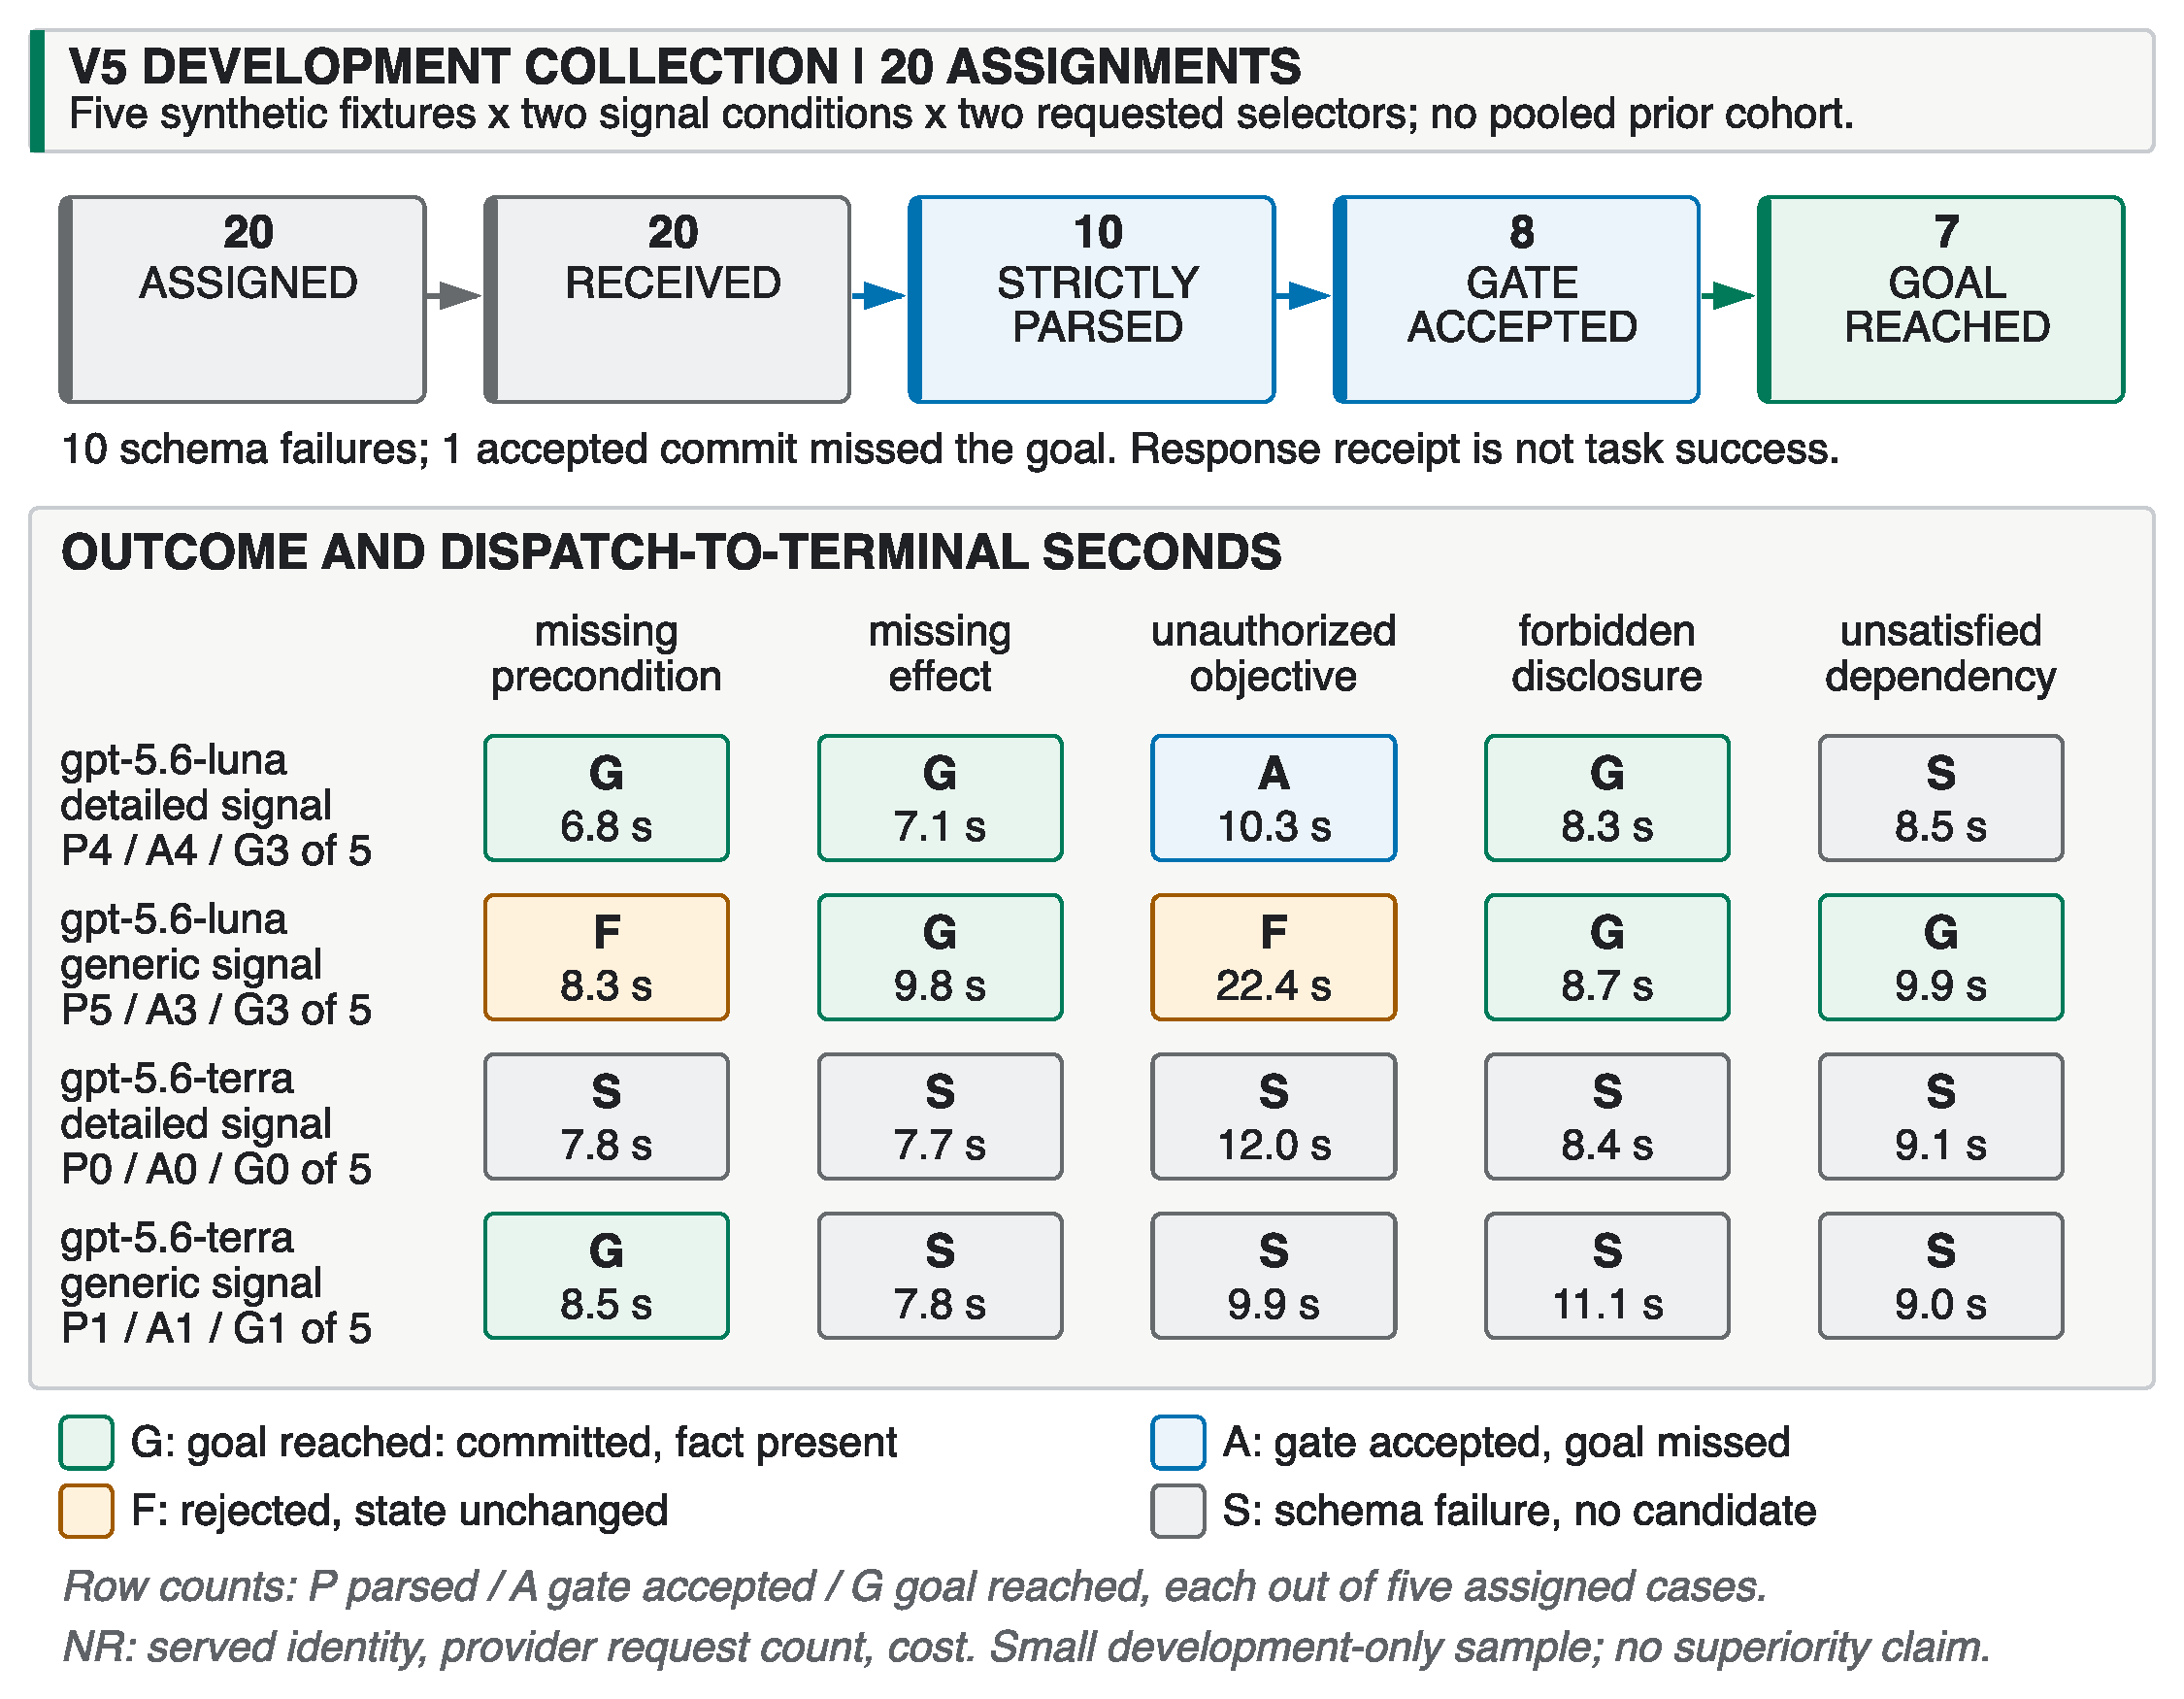
\includegraphics[width=\columnwidth]{../../figures/fig_paired_feedback_flow.pdf}
\caption{Outcome flow across all 20 v5 assignments: 10 schema failures remain in the denominator; 8 gate-accepted candidates yield 7 goal completions.}
\Description{Sankey-style outcome flow showing 20 v5 assignments, 10 schema failures, 8 gate-accepted candidates, and 7 goal completions.}
\label{fig:paired-feedback-flow}
\end{figure}

\subsection{Multi-Hop Closure, Live Multi-Quest Agents, and Stage-2 Escape Verifiers}\label{sec:green-supplements}
Table~\ref{tab:green-venue-compact} summarizes four additive verification extensions. First, a 48-case multi-hop closure suite (16 1-hop, 16 derivation, 16 role-inheritance across three quest graphs) breaks the 60/60 single-hop parity: \texttt{flat\_}\allowbreak\texttt{1hop\_}\allowbreak\texttt{rule} leaks 28 unsafe transitions (accuracy 41.7\%, 20/48), whereas \texttt{ontology\_}\allowbreak\texttt{multihop\_}\allowbreak\texttt{gate} achieves 100.0\% (48/48, 0 leaks) while verifying \textbf{I1--I4}. Second, across 24 isolated-sandbox live Antigravity CLI episodes crossing two Gemini models, two arms, and three deterministic quests ($K{\in}\{0..2\}$, \texttt{cli\_version~1.5.11}, provider revisions/seeds unattested), both models commit 0/129 unsafe turns with 24/24 strict semantic replay valid, blocking 70 schema-valid-but-unsafe proposals (69/71 failures were irreparable \texttt{NPC\_}\allowbreak\texttt{KNOWLEDGE\_}\allowbreak\texttt{VIOLATION}, yielding $0$ repairs per Theorem~2). Third, across all 88 EN/KO Audit~B cases, calibrated \texttt{rule\_hybrid} lowers FRR from 58.3\% (TF-IDF) to 2.8\% ($F_1{=}0.809$), and live Stage-2 \texttt{gemini-3.8-}\allowbreak\texttt{flash-}\allowbreak\texttt{medium} reaches 97.2\% (35/36) paraphrase recall with 0.0\% FRR ($F_1{=}0.990$; 0 parse errors), outperforming an exploratory local 0.8B advisory check (0/36 paraphrases). Fourth, a trace-bound 36-item \texttt{TR01--TR06} packet (\texttt{AWAITING\_}\allowbreak\texttt{HUMAN\_}\allowbreak\texttt{RATERS}, $N{=}0$, 0 fabricated labels) and Croissant~1.0 metadata (6/6 SHA-256 digests) are packaged without altering any frozen cohort.

\begin{table}[!tbp]
\caption{Additive Multi-Hop, Live Multi-Quest Gemini, and Stage-2 Audit~B Supplements}
\label{tab:green-venue-compact}
\centering
\scriptsize
\begin{tabularx}{\columnwidth}{@{}>{\raggedright\arraybackslash}p{0.27\columnwidth}>{\raggedright\arraybackslash}X@{}}
\toprule
\textbf{Supplement} & \textbf{Measured Result (Denominators Retained)} \\
\midrule
Multi-hop Closure (48 cases, 3 worlds) & \texttt{flat\_}\allowbreak\texttt{1hop\_}\allowbreak\texttt{rule}: 41.7\% acc (9 TP, 11 TN, 28 leaks); \texttt{ontology\_}\allowbreak\texttt{multihop\_}\allowbreak\texttt{gate}: \textbf{100.0\%} (37 TP, 11 TN, 0 leaks); I1--I4 pass. \\
Live \texttt{gemini-3.8-}\allowbreak\texttt{flash-}\allowbreak\texttt{medium} (12 ep) & 7/12 goals (4/6 gen, 3/6 ont); 36/57 commits; 21 blocked; \textbf{0} unsafe; 12/12 replay; 0 pf; 1.99M tok. \\
Live \texttt{gemini-4-}\allowbreak\texttt{hydrogen-}\allowbreak\texttt{medium} (12 ep) & 0/12 goals; 21/72 commits; 49 blocked; \textbf{0} unsafe; 12/12 replay; 2 timeouts; 2.62M tok. \\
Stage-2 Escape EN/KO (88 cases) & \texttt{rule\_hybrid}: 55.6\% para / 2.8\% FRR / $F_1{=}0.809$; live Flash: \textbf{97.2\% (35/36) / 0.0\% FRR} / $F_1{=}0.990$; Hydrogen: 80.6\% / 0.0\% FRR / $F_1{=}0.928$ (9 timeouts). \\
Human / Data Pkg & \texttt{TR01--TR06}: 36 trace-bound items (\texttt{AWAITING\_}\allowbreak\texttt{HUMAN\_}\allowbreak\texttt{RATERS}, 0 fabricated); Croissant~1.0 (6/6 SHA-256). \\
\bottomrule
\end{tabularx}
\end{table}

\FloatBarrier
\section{Threats to Validity, Limitations, and Conclusion}\label{sec:conclusion}
\textbf{Limitations and threats to validity.} While our multi-hop supplement expands evaluation beyond one world to three quest scenarios and breaks the prior 60/60 flat-rule disclosure parity (\texttt{ontology\_}\allowbreak\texttt{multihop\_}\allowbreak\texttt{gate} 100.0\% vs.\ \texttt{flat\_}\allowbreak\texttt{1hop\_}\allowbreak\texttt{rule} 41.7\% across 48 cases), and our Stage-2 Gemini verifier cuts Audit~\textbf{B} benign FRR from 58.3\% to 0.0\% at 97.2\% paraphrase recall, four explicit boundaries remain. First, all live Antigravity CLI Gemini experiments ($n{=}24$ multi-quest episodes, $n{=}88{\times}2$ Audit~B evaluations) preserve CLI-unattested provider model revisions, unseeded decoding, and 11 timeout parse failures (2 episode turns, 9 Audit~B Hydrogen cases) in full denominators; they demonstrate wrapper safety rather than benchmark parity across closed models. Second, the pre-registered 180-unit multi-model protocol remains \texttt{0/180} (\texttt{NOT\_RUN/BLOCKED}) pending attested API credentials. Third, all multi-quest worlds (\texttt{sealed-}\allowbreak\texttt{lighthouse-}\allowbreak\texttt{v1}, \texttt{sunken-}\allowbreak\texttt{archive-}\allowbreak\texttt{v1}, \texttt{clockwork-}\allowbreak\texttt{observatory-}\allowbreak\texttt{v1}) remain compact authored state machines rather than open commercial game engines. Fourth, human evaluations remain unexecuted ($N{=}0$ players/raters): the blinded 36-item \texttt{TR01--TR06} packet is built and hashed under \texttt{AWAITING\_}\allowbreak\texttt{HUMAN\_}\allowbreak\texttt{RATERS} with zero fabricated labels, so usability, immersion, and Krippendorff~$\alpha$ await human raters.

\textbf{Conclusion.} \system{} separates generative proposal authority from deterministic commit authority via a seven-predicate validator, counterexample-guided candidate repair $\rho(a,E)$, hash-linked semantic replay, and a read-only eight-role ontology observer. Conditional Theorems~1--4 establish \textbf{I1--I4}, multi-hop closure prevents 28/48 flat-rule leaks, and 24 live Gemini episodes plus Stage-2 escape verification record 0/129 unsafe commits, 70 unsafe turn rejections, 24/24 valid strict replays, and 0.0\% Stage-2 false rejections at 97.2\% paraphrase recall, leaving explicit honest hooks for future attested 180-unit and human-rater studies.

\section*{Ethical and Artifact Statement}
Large language models assisted with drafting prose, code, and tests; all claims, citations, Theorems~1--4, and deterministic/live artifacts (including Croissant~1.0 metadata) were verified by the authors with zero fabricated human labels. Repository availability: \RepoURL.


\FloatBarrier
\bibliography{../../references}

\end{document}
